\chapter{State of the Art}\label{chapter:state-of-the-art}
This chapter presents an overview of state of the art approaches to object recognition, while focusing on two families of architectures, which are motivated quite differently. Object recognition techniques based on convolutional neural networks (\emph{CNN}s) currently dominate the field, achieving state of the art performance on many datasets \cite{Diba2017WeaklySC,7506134}. CNNs however, are only loosely based on biological neurons. Spiking neural networks (\emph{SNN}s) on the other hand, try to mimic the physical properties of neurons more closely and therefore constitute biologically more plausible models \cite{Schofield20180027}. Generally speaking, CNNs may be regarded as a more engineering-based approach (or top-down), while SNNs are motivated by results from neuroscience and biology (bottom-up approach).
\section{Deep Learning for Object Recognition}
Recent years have seen a surge of interest in deep learning methods, especially in the field of computer vision. While the theory behind many deep learning methods has been around for many years, their recent success is mainly due to the availability of large labelled data sets and highly parallel computing powered by GPUs. One of the specific tasks, deep learning based methods excel at, is object recognition: the identification of objects in images or videos (cf. figure \ref{fig:cifar10}). The significantly better performance of deep neural networks over traditional machine learning methods can be explained by: (i) their hierarchical topology of parameterized non-linear processing units is a fundamentally better probabilistic model and prior for real world data leading to better generalization and (ii) they automatically find good features to extract based on the training data.
\begin{figure}
    \centering
\begin{tikzpicture}
  \node[anchor=south west,inner sep=0] at (0,0) {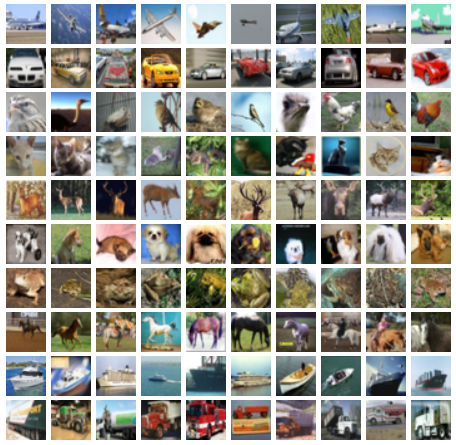
\includegraphics{figures/cifar10.png}};
  \node[anchor=west] at (-2.5,8.9) {Airplane};
  \node[anchor=west] at (-2.5,7.95) {Automobile};
  \node[anchor=west] at (-2.5,7.05) {Bird};
  \node[anchor=west] at (-2.5,6.1) {Cat};
  \node[anchor=west] at (-2.5,5.2) {Deer};
  \node[anchor=west] at (-2.5,4.25) {Dog};
  \node[anchor=west] at (-2.5,3.35) {Frog};
  \node[anchor=west] at (-2.5,2.45) {Horse};
  \node[anchor=west] at (-2.5,1.5) {Ship};
  \node[anchor=west] at (-2.5,.55) {Truck};
\end{tikzpicture}\noindent
\caption[CIFAR-10 classes and sample images]{Sample images from the CIFAR-10 \cite{cifar10} dataset and their corresponding classes. CIFAR-10 consists of 6000 images at 32 by 32 pixels for each of the 10 classes. Datasets such as this are often used as a benchmark to evaluate the performance of novel deep learning architectures for image recognition. This is done by using a subset of the dataset to train the neural network. The remainder of the images, which the network has not seen before, are used to evaluate the accuracy.}\label{fig:cifar10}
\end{figure}
The potential applications for a robust image classification system are myriad and range from automated driving and image-based diagnosis to robot vision and many more. As deep learning is currently the best candidate for such a system, it is well worth exploring.
\subsection{Convolutional Neural Networks}
CNN architectures are generally distinguished by their use of specific types of neuron-layers, namely, convolutional, pooling and fully connected layers. While wildly different network topologies may be found in literature, characterized by their use of skip connections, number of layers, number of paths etc., CNNs can always be reduced to these three basic layer types.
\subsubsection{Fully Connected Layer}
Each neuron in a fully connected layer is connected to all the activations in the previous layer. The activation of a single neuron (cf. figure \ref{fig:neuron}) is calculated by applying a nonlinearity to the weighted sum of its inputs and a bias.
\begin{align}
    h = g\qty(\sum_i w_i x_i +b)
    \label{eq:neuron}
\end{align}
\begin{figure}
    \centering
\begin{tikzpicture}
  \node[anchor=south west,inner sep=0] at (0,0) {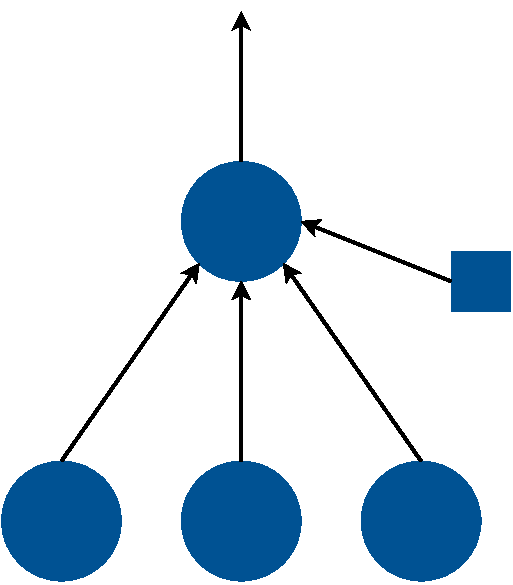
\includegraphics[scale=.5]{figures/Neuron.pdf}};
  \node[anchor=west] at (.2,1.8) {$w_1$};
  \node[anchor=west] at (1.3,1.8) {$w_2$};
  \node[anchor=west] at (2.3,1.8) {$w_3$};
  \node[anchor=west] at (4.3,2.6) {$b$};
  \node[anchor=west] at (.2,-.5) {$x_1$};
  \node[anchor=west] at (1.75,-.5) {$x_2$};
  \node[anchor=west] at (3.3,-.5) {$x_3$};
  \node[anchor=west] at (1.3,4.2) {$h$};
\end{tikzpicture}
\caption[Illustration of an artificial neuron with three input connections]{Illustration of an artificial neuron with three input connections. Artificial neurons constitute the basic non-linear computational units of neural networks. The neuron receives the activations of three lower level neurons weighted by the learnable $w_i$ as well as a learnable bias $b$. After applying the nonlinearity (also known as activation function), the neuron outputs its activation $h$ as in equation  \ref{eq:neuron}}\label{fig:neuron}
\end{figure}\noindent
With the nonlinear function $g$, the learnable weights $w_i$, the input activations $x_i$ and the learnable bias $b$. In the case of a fully connected layer, the activations can be computed using matrix multiplication. In tensor notation this may be written as:
\begin{align}
    \vb{h_l} = g_l\qty(\vb{W^T_l\vb{h_{l-1}}}+\vb{b_l}).
\end{align}
With $N_l$ denoting the number of neurons in layer $l$, $\vb{W_l}$ is an $N_{l-1}\cp N_l$ dimensional weight matrix, $b_l$ an $N_l$ dimensional vector and $g_l$ the $N_l$ dimensional vectorized activation function of layer $l$.
\begin{align}
    g_l(\vb{x}) = \qty(g_l(x_1),...,g_l(x_{N_l}))^T
\end{align}
The computational power of neural networks is shown by the universal approximation theorem. The theorem states, that networks with a single hidden layer (cf. figure \ref{fig:fully-connected}) containing a finite number of neurons can approximate arbitrary continuous functions on compact subsets of $\mathbb{R}^n$ \cite{univ-approx-1,univ-approx-2}.
\begin{figure}
    \centering
\begin{tikzpicture}
  \node[anchor=south west,inner sep=0] at (0,0) {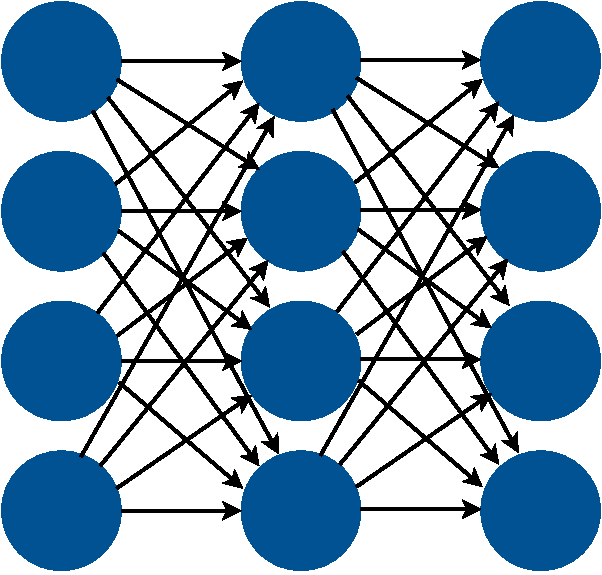
\includegraphics[scale=.5]{figures/FullyConnected.pdf}};
  \node[anchor=west] at (.2,-.5) {$h_0$};
  \node[anchor=west] at (2.3,-.5) {$h_1$};
  \node[anchor=west] at (4.3,-.5) {$h_2$};
\end{tikzpicture}
\caption[Illustration of fully connected layers]{Illustration of a fully connected neural network as a directed graph with input layer $h_0$ and output layer $h_2$. Layers between the input and output layer are usually referred to as \emph{hidden} layers. Note that the biases are not explicitly shown.}\label{fig:fully-connected}
\end{figure}\noindent
\subsubsection{Convolutional Layer}
In a convolutional layer, the activities of the input layer are convolved with a number of trainable kernels so as to create the same number of feature maps. In computer vision it is common to view the layer's neurons as two-dimensional grids of neurons arranged in channels (cf. figure \ref{fig:2dconvolution}). These grids correspond to pixels and color channels in the case of the input layer or activities (feature maps) resulting from convolution with different kernels in the case of intermediate convolutional layers. For a feature kernel $F_{m,n}^l$ of size $M_l\cp M_l$ and an input layer $l-1$ with $N_{l-1}\cp N_{l-1}$ neurons, the corresponding feature map activities of layer $l$ are computed as
\begin{align}
    h^l_{m,n} = g_l\qty(\sum_{m'}^{M_l}\sum_{n'}^{M_l}F_{m',n'}^l h_{m+m',n+n'}^l+b_l).
    \label{eq:2dconv}
\end{align}
This is the same as a two-dimensional discrete cross correlation.
\begin{align}
    (f \star g)[n]\ \stackrel{\mathrm{def}}{=} \sum_{m=-\infty}^{\infty} f^*[m]\ g[m+n]
\end{align}
Where $f^*$ is the complex conjugate of the discrete function $f$. Strictly speaking, the use of the term \emph{convolution} in neural network literature is therefore a misnomer, as either the filter or the image (or feature map) would have to be flipped before the operation. However, as the weights of the kernel are actually learned by the network, the result will be the same. 

For a 2D single channel input layer of size $N_0\cp N_0$, the number of trainable parameters for a convolutional layer with a single $M\cp M$ filter is $M^2 + 1$ for the kernel weights and bias respectively, compared to $N_0^2N_1^2+N_1^2$ for a fully connected layer of size $N_1\cp N_1$. The sparsity in learnable parameters in convolutional layers compared to fully connected layers (cf. fig \ref{fig:convolutional}) is often referred to as \emph{weight sharing} (an entire channel \emph{shares} the weights of a single kernel).

In the case of multiple input channels, the kernels actually extend through the whole depth of the input layer's volume. Equation \ref{eq:2dconv} can be extended to accommodate multiple input channels and feature kernels. The activities of feature map $k$ in layer $l$ are then computed as
\begin{align}
    h^l_{k,m,n} = g_l\qty(\sum_{k'}^{K_{l-1}}\sum_{m'}^{M_l}\sum_{n'}^{M_l}F_{k,k',m',n'}^l h_{k',m+m',n+n'}^l+b_{l,k}).
    \label{eq:conv-multilayer}
\end{align}
With $K_l$ the number of channels in layer $l$. Most deep learning frameworks offer additional hyperparameters for convolutional layers, like stride and zero padding. Zero padding adds additional rows and columns of zero-activities around the input layer channels, effectively allowing the output feature maps to have the same size (i.e. height and width, depth is determined by the number of kernels) as the unpadded input layer. Stride on the other hand defines the integer value by which the kernels are moved during convolution. This can be used to keep the receptive fields from overlapping too much. Equation \ref{eq:conv-multilayer} is easily extended to take the stride $S_l$ of layer $l$ into consideration.
\begin{align}
    h^l_{k,m,n} = g_l\qty(\sum_{k'}^{K_{l-1}}\sum_{m'}^{M_l}\sum_{n'}^{M_l}F_{k,k',m',n'}^l h_{k',S_l m+m',S_l n+n'}^l+b_{l,k})
\end{align}
The spatial dimension of this feature map can be computed as a function of the input layer size $N_{l-1}\cp N_{l-1}$ and the amount of zero padding $P_l$.
\begin{align}
    N_l = \frac{N_{l-1}-M_l+2P_l}{S_l}+1
\end{align}
\begin{figure}
    \centering
\begin{tikzpicture}
  \node[anchor=south west,inner sep=0] at (0,0) {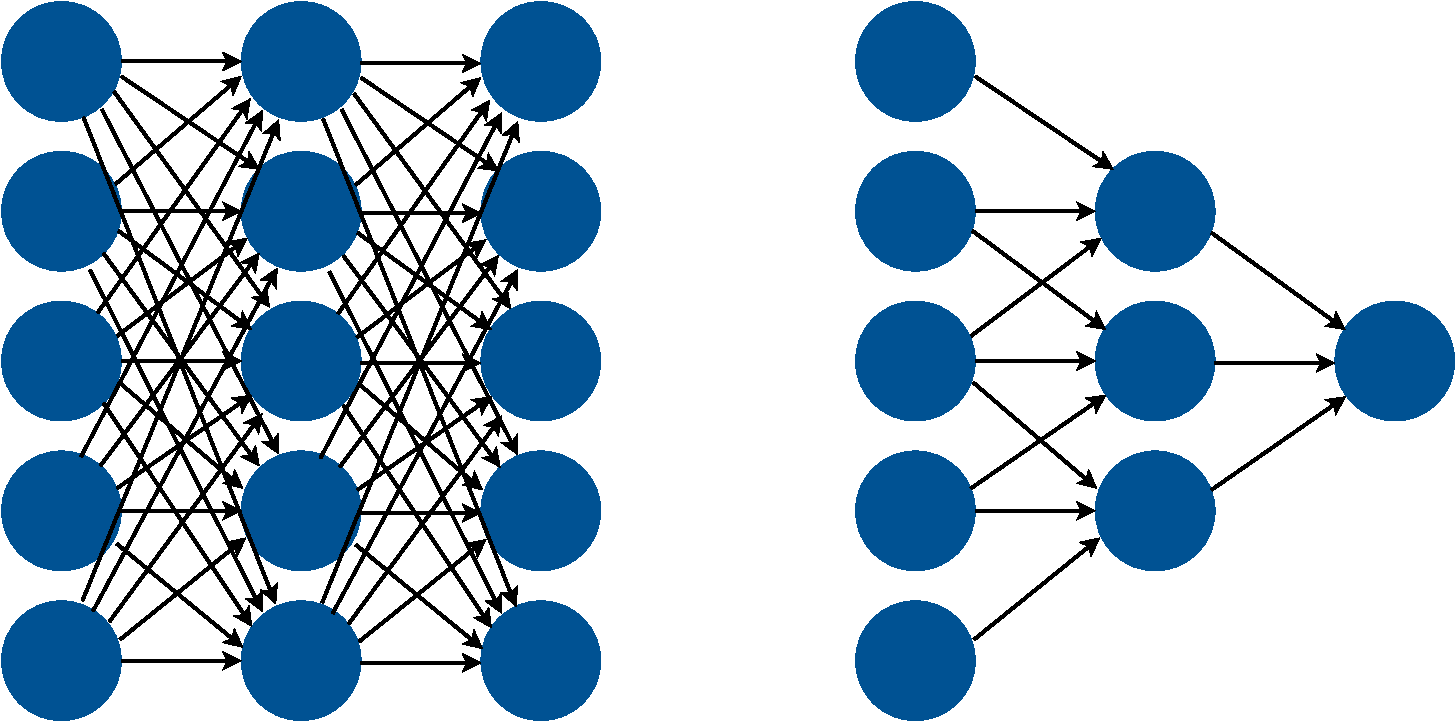
\includegraphics[scale=.5]{figures/Convolutional.pdf}};
  \node[anchor=west] at (.2,-.5) {$h_0$};
  \node[anchor=west] at (2.3,-.5) {$h_1$};
  \node[anchor=west] at (4.3,-.5) {$h_2$};
  \node[anchor=west] at (7.5,-.5) {$h'_0$};
  \node[anchor=west] at (9.6,-.5) {$h'_1$};
  \node[anchor=west] at (11.6,-.5) {$h'_2$};
\end{tikzpicture}
\caption[Illustration of convolutional layers]{Illustration of fully connected layers compared to convolutional layers, making apparent the sparsity of the latter relative to the former. The convolutional layers $h'_1$ and $h'_2$ perform a 1D convolution with a filter of size $3$. Note that due to weight sharing the number of weight parameters between $h'_0$ and $h'_1$ is actually only $3$. Also note, that convolution reduces the number of neurons (or pixel resolution in the case of an image). For an input layer with $N$ neurons and a filter kernel of size $M$ the number of neurons in the convolutional layer computes as $N-M+1$. }\label{fig:convolutional}
\end{figure}\noindent
\begin{figure}
    \centering
\begin{tikzpicture}
  \node[anchor=south west,inner sep=0] at (0,0) {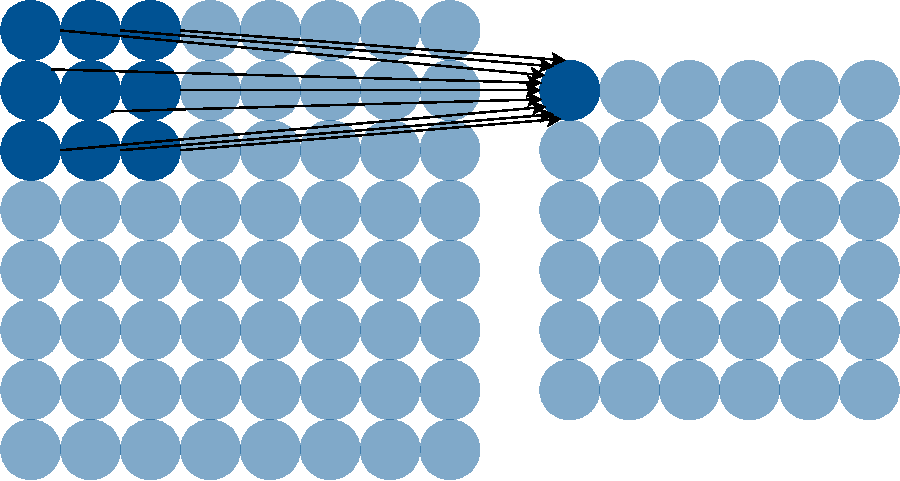
\includegraphics[scale=.5]{figures/2DConvolution.pdf}};
  \node[anchor=west] at (.4,4.5) {$M_l$};
  \node[anchor=west] at (-1,3.3) {$M_l$};
  \node[anchor=west] at (1.8,-.5) {$h_0$};
  \node[anchor=west] at (5.8,-.5) {$h_1$};
\end{tikzpicture}
\caption[Illustration of receptive field in 2D convolutional layer]{Illustration of a 2D convolution with a kernel of size $M_l\cp M_l$. As the resulting feature map $h_1$ has a lower resolution than $h_0$, applying a convolutional layer is sometimes also referred to as downsampling. For an input layer with $N\cp N$ neurons, the feature map's size is computed as $(N-M_l+1)\cp (N-M_l+1)$. The area comprised of the input neurons that are used to calculate the activity of a feature map neuron (highlighted neurons in layer $h_0$) are known as that neuron's \emph{receptive field}.}\label{fig:2dconvolution}
\end{figure}\noindent
\subsubsection{Pooling Layer}
Pooling is a form of sub- or downsampling using a sliding window similar to convolution. Most often the stride is set equal to the window size - that way the windows don't overlap. An operator is applied to each window, which selects a single neuron. Common operators are maximum, average or $L_2$-Norm. The pooling is applied to each channel and leads to a reduction in the spatial dimensions. This reduction corresponds to a loss of information or reduction in degrees of freedom and therefore reduces the amount of computation required as well as the possibility of overfitting. The choice of pooling operator has a profound effect on the generalization and speed of convergence of CNNs and recently maximum pooling has proven to be the most successful method \cite{pooling1,pooling2}.
\begin{figure}
    \centering
\begin{tikzpicture}
  \node[anchor=south west,inner sep=0] at (0,0) {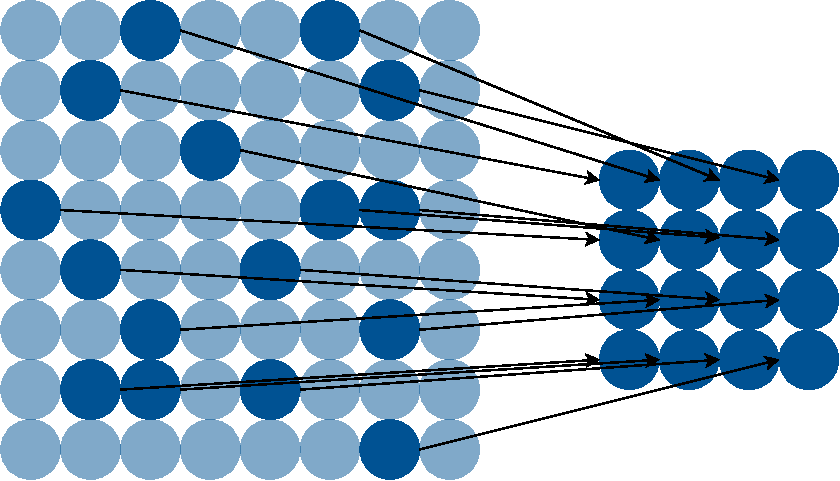
\includegraphics[scale=.5]{figures/Pooling.pdf}};
  \node[anchor=west] at (1.8,-.5) {$h_0$};
  \node[anchor=west] at (5.8,-.5) {$h_1$};
  \draw [decorate,decoration={brace,amplitude=5pt},xshift=-4pt,yshift=0pt]
(-0.1,3.1) -- (-0.1,4.05) node [black,midway,xshift=-0.6cm] {$M_l$};
  \draw [decorate,decoration={brace,amplitude=5pt},xshift=-4pt,yshift=0pt]
(.15,4.3) -- (1.2,4.3) node [anchor=south,midway,yshift=1] 
{$M_l$};
\end{tikzpicture}
\caption[Illustration of a pooling layer]{Illustration of a pooling layer. The pooling uses a $2\cp 2$ window with stride 2 to segment the input layer into non-overlapping tiles. An operator (e.g. maximum) is applied to each $2\cp 2$ segment to select a single neuron (the highlighted neurons in layer $h_0$). The activities of the selected neurons are aranged in a new layer $h_1$ of size $\frac{N_{l-1}}{M_l}\cp \frac{N_{l-1}}{M_l}$ with $M_{l}\cp M_{l}$ and $N_{l-1}\cp N_{l-1}$ the size of the window the input layer respectively.}\label{fig:pooling}
\end{figure}\noindent
\subsubsection{CNN Architecture}
The key idea behind the combination of these three types of layers is, that essential visual features such as edges and corners within a convolutional layer's receptive field are combined to form higher level features such as shapes by subsequent convolutional layers. In between these convolutions, pooling operations select the most salient features and reduce the computational size of the network. The convolutional kernels are effectively trainable feature detectors and due to weight sharing and pooling naturally incorporate a measure of translational invariance. This hierarchical organization of receptive fields is similar in structure to the mammalian visual cortex \cite{cat-brain} and sometimes CNNs are seen to be directly derived from it \cite{Fukushima1980,lecun2015deep}. More often than not however, the use of convolutional layers with weight sharing is motivated as a means to achieve translational equivariance and faster computation compared to fully connected layers \cite{Goodfellow-et-al-2016,7298668,7298594}. Finally, fully connected layers are placed on top of the network in order to perform high level inference (cf. figure \ref{fig:cnn-arch}). A CNN's architecture is therefore largely defined by its \emph{hyperparameters}: the number and types of layers and their connections. The number of stacked layers is often referred to as the network's depth. Current networks often employ multiple paths and skip connections (i.e. a layer's output not only flows to its direct descendent, but skips several layers) allowing for topologies several hundred layers deep, hence \emph{deep learning} \cite{huang2017densely,szegedy2017inception,xie2017aggregated,wang2015towards}.

\begin{figure}
    \centering
\def\svgwidth{\textwidth}
\import{figures/}{AlexNet.pdf_tex}
%\input{figures/AlexNet.tex}
\caption[Illustration of a typical CNN architecture]{Illustration of a typical CNN architecture for object recognition. Note that the feature maps of the first convolutional layer extracted elementary features like edges. The last layer's neurons correspond to the trained classes, while the output neuron with the highest probability is picked as the network's prediction (highlighted in red).}\label{fig:cnn-arch}
\end{figure}\noindent
\subsubsection{Training}
For object recognition, the output of the final layers are the class probabilities. This is achieved by applying a normalizing activation function to the the output of the last layer, such as the \emph{softmax} function. In case of the softmax function, the network's prediction $y_k\qty(\vb{a})$ for the class $k$ thus becomes
\begin{align}
    y_k\qty(\vb{a}) = \frac{\exp(a_k)}{\sum_{k'}^K \exp(a_{k'})}.
\end{align}
With $\vb{a}=(a_1,...,a_K)^T$ the linear activities of the last layer's neurons (in machine learning literature often referred to as \emph{logits}) and $K$ the number of classes.
\subsection{Spiking Neural Networks}
\section{Limits of Deep Learning Approaches}